\documentclass{article}

\usepackage{graphicx}
\usepackage[margin=10pt,font=small,labelfont=bf]{caption}
\usepackage{subcaption}

\graphicspath{ {./../images} }

\begin{document}
\section*{Screenshots}

\begin{figure}[htp]
    \centering
    \begin{subfigure}{.5\textwidth}
        \centering
        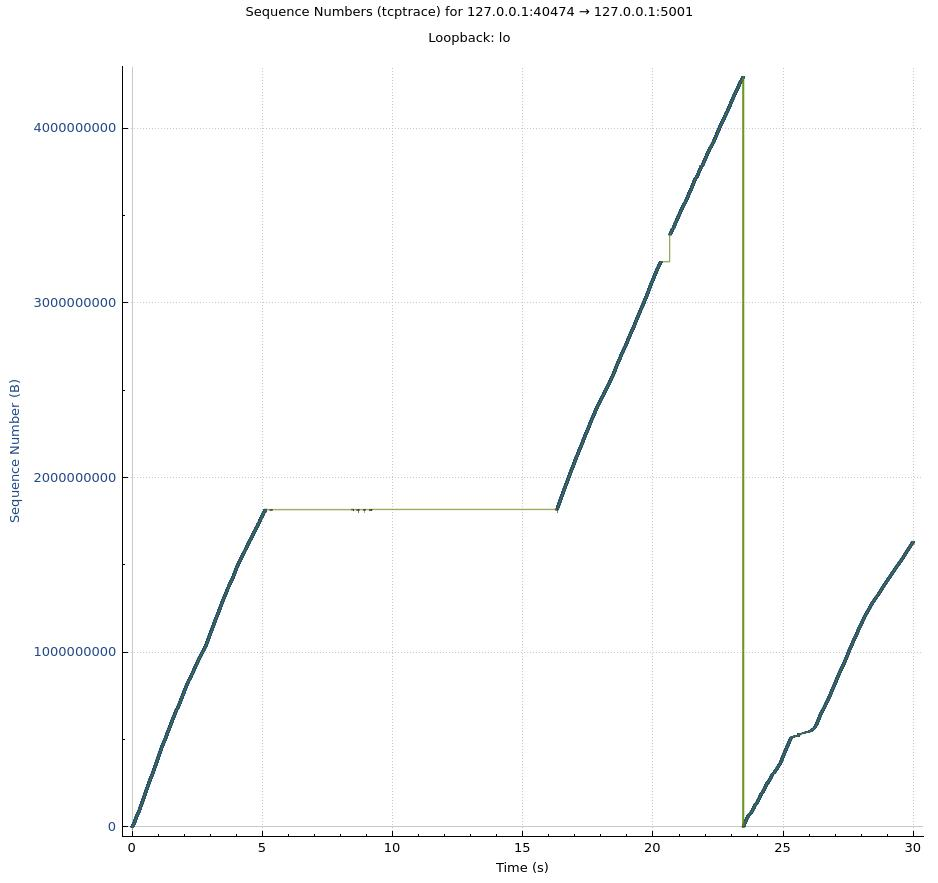
\includegraphics[width=\linewidth]{tcptrace}
        \caption{Tcptrace}
    \end{subfigure}%
    \begin{subfigure}{.5\textwidth}
        \centering
        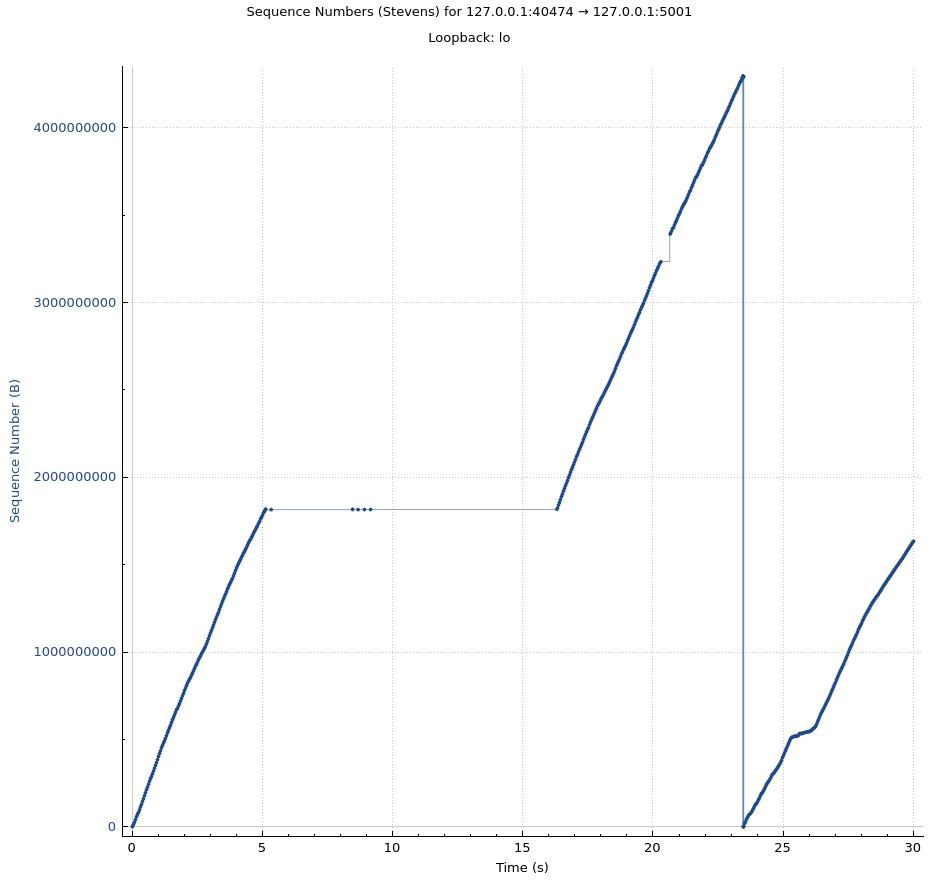
\includegraphics[width=\linewidth]{stevens}
        \caption{Stevens}
    \end{subfigure}
    \caption{Reno}
\end{figure}

\begin{figure}[htp]
    \centering
    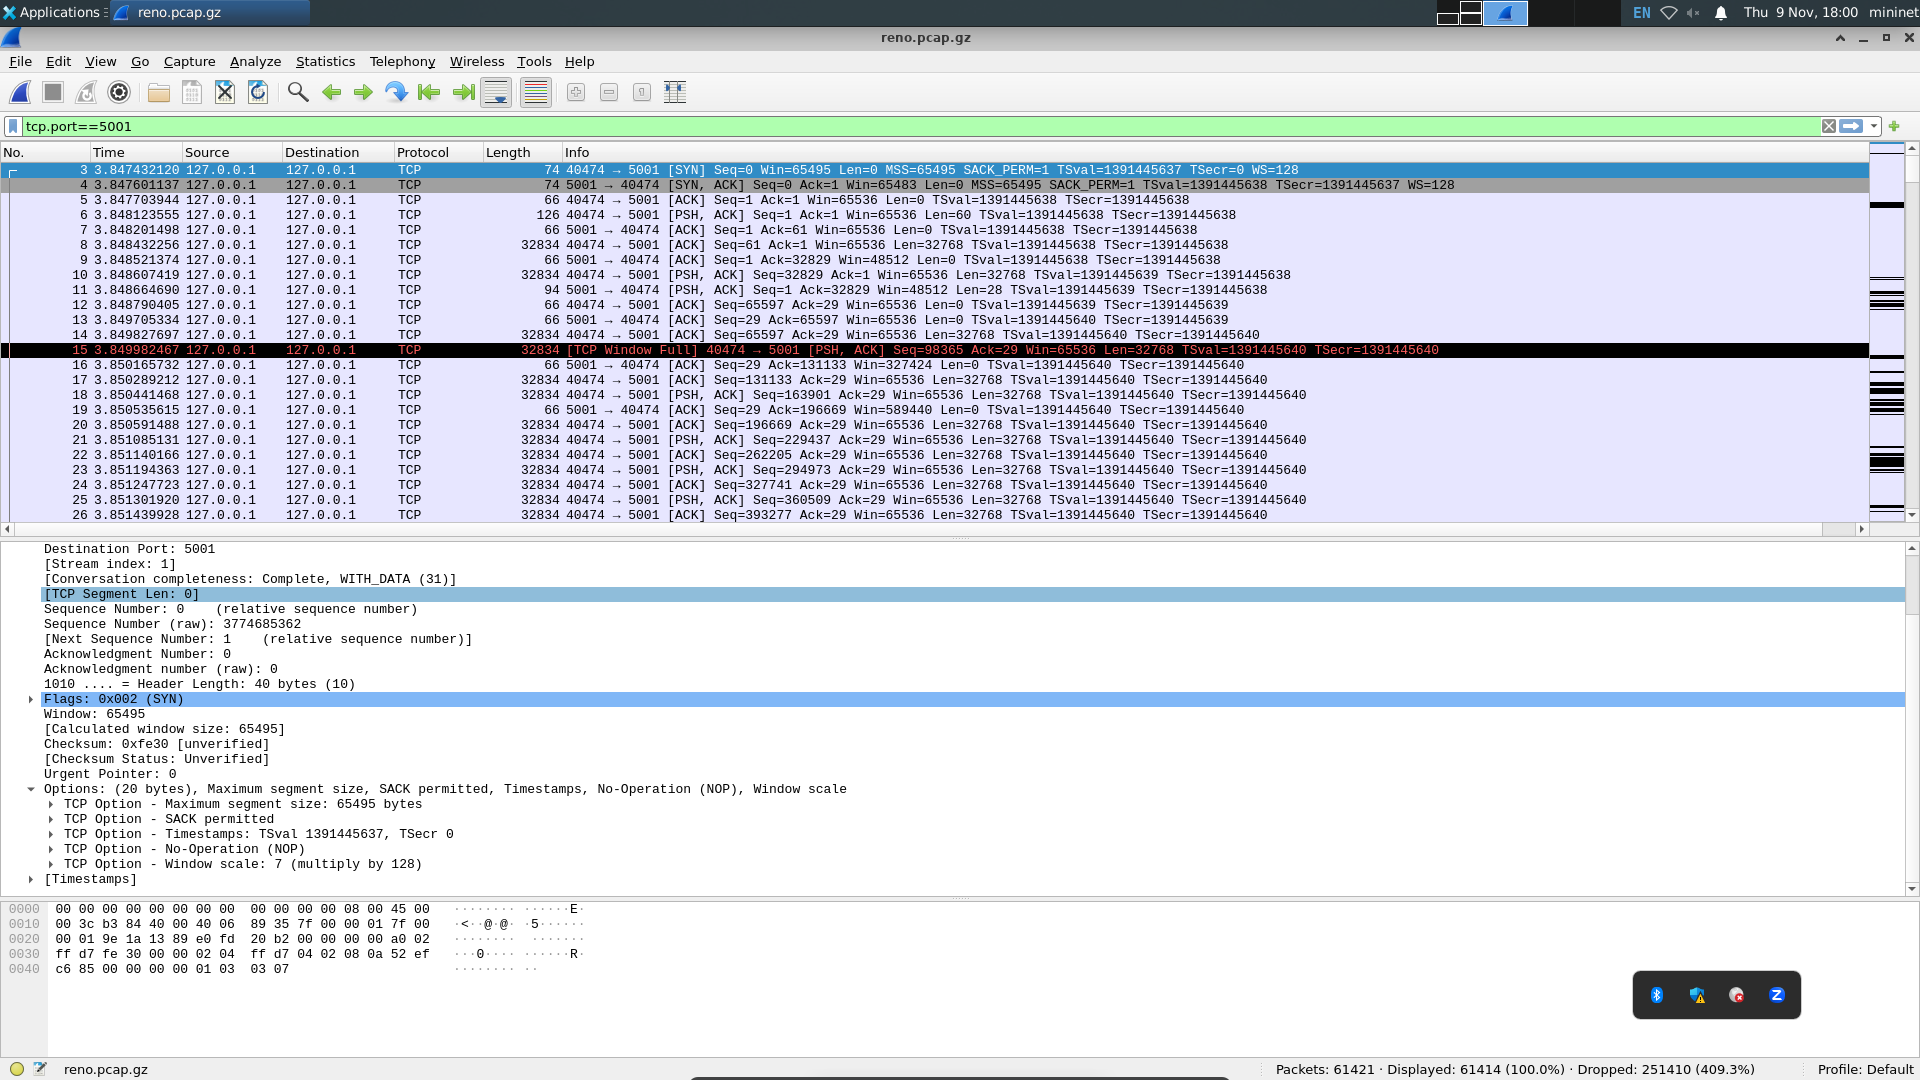
\includegraphics[width=.9\textwidth]{screenshot}%
    \caption{Terminals}
\end{figure}

\clearpage
\section*{Questions}
\subsection*{No Loss}
\noindent
On the time-sequence graph (tcp trace), identify the regions of slow start and
congestion avoidance.

Almost imidetly 

\noindent
How many duplicate ACK did you capture before the TCP retransmission?

\noindent
What is the meaning of `SACK' options in the TCP option?

\noindent
What is the meaning of the number in the `SACK' option? (the number in the red
rectangle in the below figure)

\noindent
Did you see any sequence number of the afterward TCP packet stay in that SACK range? If


\end{document}